This exercise focuses on histogram equalization, which is a method of contrast adjustment in images. Many images are taken in the High Dynamic Range (HDR) format, enabling devices to capture a wider range og colors. When we display images we can only show them in the 8 bit range meaning, when displaying a HDR image using float values, a lot of details are lost when mapped. When mapped directly an image consisting of many dark colors in a narrow range, may resulting in an image as seen on \cref{fig:ex3-before}.
Therefor when mapping an image from the float range to the 8 bit range, a histogram equalization may be necessary. In histogram equalization the pixels are scales so the whole range of an image is used equally, as represented on \cref{fig:histogram_eq}. 

\begin{figure}[ht]
	\centering
	\begin{subfigure}{.5\textwidth}
		\centering
		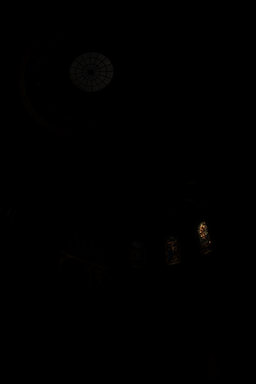
\includegraphics[width=0.5\textwidth]{figs/exercises/ex3/memorial_raw.png}
		\caption{Before}
		\label{fig:ex3-before}
	\end{subfigure}%
	\begin{subfigure}{.5\textwidth}
		\centering
		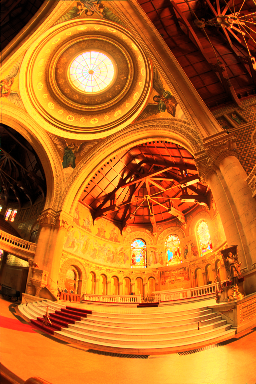
\includegraphics[width=0.5\textwidth]{figs/exercises/ex3/memorial_gold.png}
		\caption{After}
		\label{fig:ex3-after}
	\end{subfigure}
	\caption{Picture before and after histogram equalization}
	\label{fig:ex3}
\end{figure}  

\begin{figure}[ht]
	\centering
	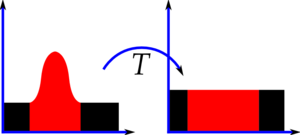
\includegraphics[width=0.5\textwidth]{figs/exercises/ex3/histogram_eq.png}
	\caption{Histograms of an image before and after equalization \cite{wiki:hist_eq}}	\label{fig:histogram_eq}
\end{figure}  

Instead of working with all the channels in the RGB space, the image is converted to YUV space, as only one channel needs to be equalized, namely the Chrominance-Luminance. The task of the exercise is to calculate the cumulative distribution of the luminance channel. This can be done through 4 steps, as presented below.
\begin{enumerate}
	\item[\textbf{Step 1}]
	Find the minimum and maximum value in the luminance channel. This can be done through two different reduction algorithms, having the binary associative operator maximum or max and minimum or min respectively. One should also consider the size of the luminance array, as it is larger than the  thread block size.  
	\item[\textbf{Step 2}]
	Find the range of the luminance values, which is the difference between the minimum and maximum values calculated in step 1. 
	\item[\textbf{Step 3}]
	Calculate a histogram of the values in the luminance array. the number of pixels in each image pixel range needs to be calculated so the image histogram can be found. The way the bin for the histogram is chosen is through the equation \cref{eq:bin}.
	
	\begin{equation}
	\label{eq:bin}
		bin = \frac{(lum[i]-lumMin)}{lumRange}*numBins
	\end{equation}
	
	When running the histogram in parallel, one should consider the race condition scenario where multiple threads may try to write to the same address. This scatter operation, can be solved, using e.g. atomics, but more clever and efficient methods may be used. 
	\item[\textbf{Step 4}]
	Lastly the cumulative histogram is calculated using a scan operation on the histogram. The scan should be an exclusive scan, so the scan algorithm by Blelloch may be a good choice.  
\end{enumerate}  